\documentclass[12pt]{article}

\usepackage{amsmath}
\usepackage{array}
\usepackage{caption}
\usepackage[top=1in, bottom=1in, left=0.75in, right=0.75in]{geometry}
\usepackage{graphicx}
\usepackage[colorlinks=true, allcolors=blue]{hyperref}
\usepackage[utf8]{inputenc}
\usepackage{multirow}
\usepackage{pdfpages}
\usepackage[section]{placeins}

\graphicspath{{./figures/}}

\begin{document}

\begin{titlepage}
  \begin{center} \LARGE
    \vspace*{1.5in}

    ECE 272 Lab 1

    Fall 2018

    \vfill

    Basic Combinational Logic and the DE10-Lite

    Phi Luu

    \vfill

    October 3\textsuperscript{th}, 2018

    Grading TA: Edgar Perez

    Lab Partner: Benjamin Geyer

    \vspace{1.5in}
  \end{center}
\end{titlepage}

%%%%%%%%%%%%%%%%%%%%%%%%%%%%%%%%%%%%%%%%%%%%%%%%%%%%%%%%%%%%%%%%%%%%%%%%%%%%%%%%
% Introduction
%%%%%%%%%%%%%%%%%%%%%%%%%%%%%%%%%%%%%%%%%%%%%%%%%%%%%%%%%%%%%%%%%%%%%%%%%%%%%%%%
\section{Introduction}

The purpose of this lab is to learn how to use Quartus Prime and the MAX 10 DE10-Lite. With these software and hardware tools, we can verify the properties of combinational logic design. Throughout this lab, we will learn how to construct a combinational logic schematic and program this schematic into the DE10-Lite using Quartus Prime.

Most digital electronic implementations have moved towards Programmable Logic Devices (PLD). PLD can be classified into two following categories:

\begin{itemize}
  \item \textit{Programmable Logic Arrays} (PLA) have fixed hardware-defined logic gates whose connections are configurable.
  \item \textit{Complex Programmable Logic Devices} (CPLD) use a Hardware Description Language (HDL) to program both the connections of the logic gates and the logic gates themselves.
  \item \textit{Field-Programmable Gate Arrays} (FPGA) is a subset of CPLD.
\end{itemize}

The MAX 10 DE10-Lite is an FPGA, which means it will allow us to build and program highly customizable circuits throughout this course without using excessive electronic hardware.

%%%%%%%%%%%%%%%%%%%%%%%%%%%%%%%%%%%%%%%%%%%%%%%%%%%%%%%%%%%%%%%%%%%%%%%%%%%%%%%%
% Design
%%%%%%%%%%%%%%%%%%%%%%%%%%%%%%%%%%%%%%%%%%%%%%%%%%%%%%%%%%%%%%%%%%%%%%%%%%%%%%%%
\section{Design}

\begin{figure}[h]
  \centering
  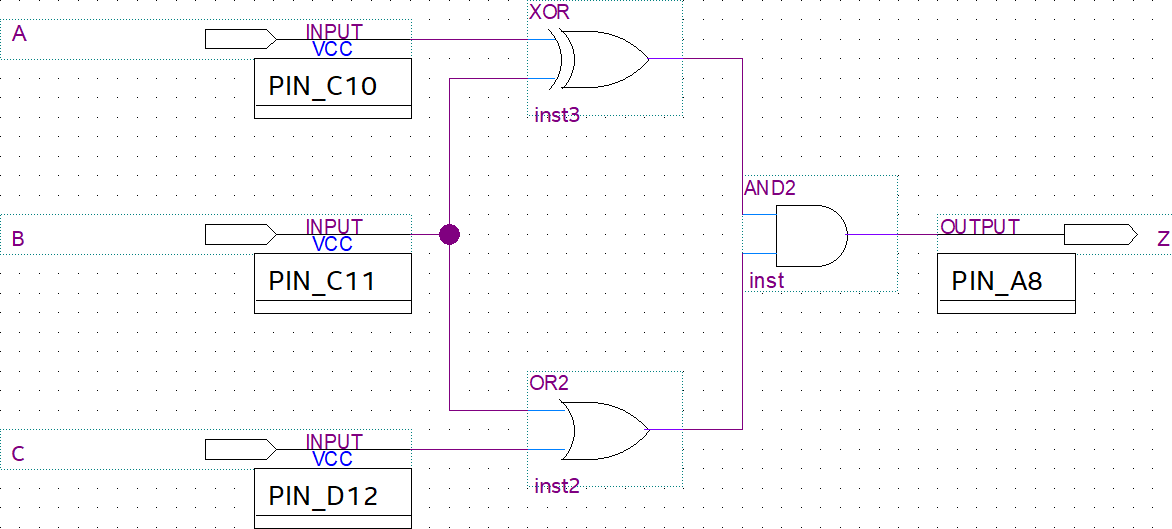
\includegraphics[width=\textwidth]{schematic.png}
  \caption{The schematic design of lab 1}
  \label{figure:1}
\end{figure}

Figure~\ref{figure:1} above shows a schematic constructed in Quartus Prime. The digital circuit includes a two-input XOR gate, a two-input OR gate, and a two-input AND gate. The output of the circuit is determined by the combination of these three gates, and the truth table of each gate is as follows:

\begin{table}[h]
  \centering
  \begin{tabular}{ | c | c | c || c | c | c || c | c | c | }
  \hline
  $\mathbf{A}$ & $\mathbf{B}$ & $\mathbf{A \textbf{ XOR } B}$ & $\mathbf{A}$ & $\mathbf{B}$ & $\mathbf{A \textbf{ OR } B}$ & $\mathbf{A}$ & $\mathbf{B}$ & $\mathbf{A \textbf{ AND } B}$ \\ \hline
  0            & 0            & 0                             & 0            & 0            & 0                            & 0            & 0            & 0                             \\ \hline
  0            & 1            & 1                             & 0            & 1            & 1                            & 0            & 1            & 0                             \\ \hline
  1            & 0            & 1                             & 1            & 0            & 1                            & 1            & 0            & 0                             \\ \hline
  1            & 1            & 0                             & 1            & 1            & 1                            & 1            & 1            & 1                             \\ \hline
  \end{tabular}
  \caption{Truth tables of two-input gates XOR, OR, and AND, respectively}
  \label{table:1}
\end{table}

\newpage

Figure~\ref{figure:2} below shows the block diagram based on which the switches and the LEDs are mapped.

\begin{figure}[h]
  \centering
  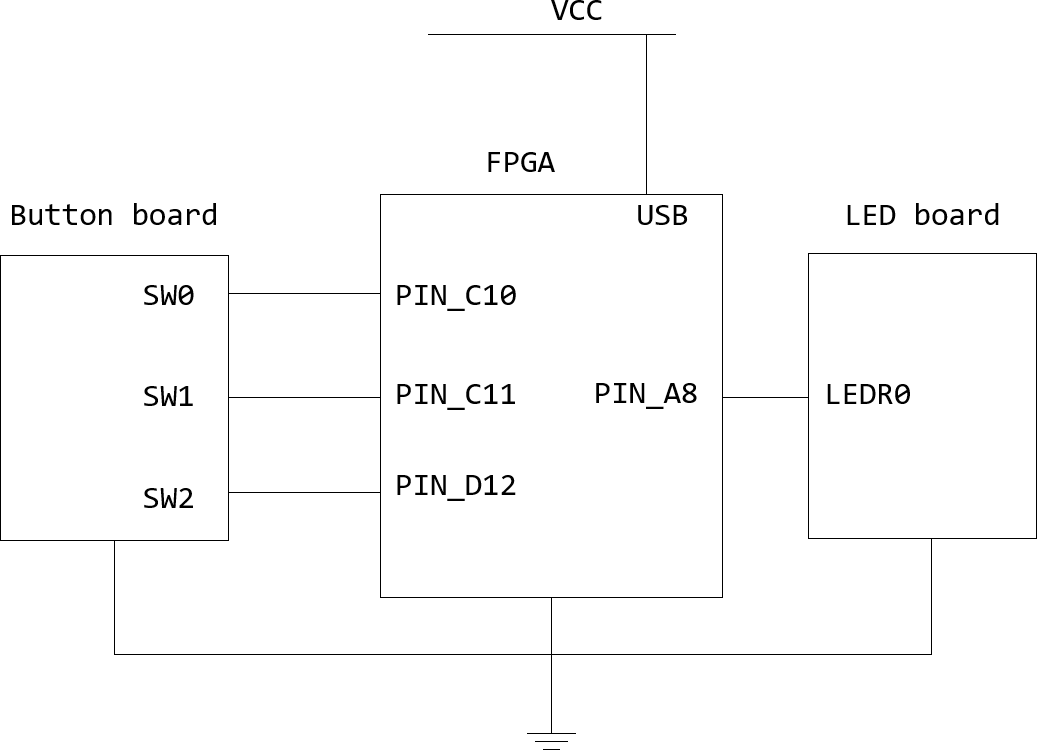
\includegraphics[width=0.75\textwidth]{block_diagram.png}
  \caption{The block diagram designed for this lab, showing the pin mapping}
  \label{figure:2}
\end{figure}

We assign the inputs A, B, and C and the output Z in the Assignment Editor of Quartus Prime, similarly to Table~\ref{table:2} below.

\begin{table}[h!]
  \centering
  \begin{tabular}{ | l | l | }
  \hline
                      & \textbf{FPGA PIN} \\ \hline
  \textbf{INPUT A}  & PIN\_C10           \\ \hline
  \textbf{INPUT B}  & PIN\_C11           \\ \hline
  \textbf{INPUT C}  & PIN\_D12           \\ \hline
  \textbf{OUTPUT Z} & PIN\_A8            \\ \hline
  \end{tabular}
  \caption{Pin assignments, connecting the schematic with the DE10-Lite}
  \label{table:2}
\end{table}

\newpage

%%%%%%%%%%%%%%%%%%%%%%%%%%%%%%%%%%%%%%%%%%%%%%%%%%%%%%%%%%%%%%%%%%%%%%%%%%%%%%%%
% Results
%%%%%%%%%%%%%%%%%%%%%%%%%%%%%%%%%%%%%%%%%%%%%%%%%%%%%%%%%%%%%%%%%%%%%%%%%%%%%%%%
\section{Results}

\begin{table}[h]
  \centering
  \begin{tabular}{ | c | c | c | c | c | }
  \hline
  \textbf{A} & \textbf{B} & \textbf{C} & \textbf{EXPECTED Z} & \textbf{ACTUAL Z} \\ \hline
  0          & 0          & 0          & 0                   & 0                 \\ \hline
  0          & 0          & 1          & 0                   & 0                 \\ \hline
  0          & 1          & 0          & 1                   & 1                 \\ \hline
  0          & 1          & 1          & 1                   & 1                 \\ \hline
  1          & 0          & 0          & 0                   & 0                 \\ \hline
  1          & 0          & 1          & 1                   & 1                 \\ \hline
  1          & 1          & 0          & 0                   & 0                 \\ \hline
  1          & 1          & 1          & 0                   & 0                 \\ \hline
  \end{tabular}
  \caption{Truth table of the final results}
  \label{table:3}
\end{table}

Shown above in Table~\ref{table:3} is the outcome of this lab. A $\mathbf{0}$ in an input value means the corresponding switch is \textbf{not pressed} (or is \textbf{toggled off}). Conversely, a $\mathbf{1}$ in input value means the corresponding switch is \textbf{pressed} (or is \textbf{toggled on}). This binary concept is also similar with the output: the corresponding LED will turn \textbf{off} if the output is $\mathbf{0}$ and will turn \textbf{on} if the output is $\mathbf{1}$.

Since the actual outputs of Z matched their expected values, the logic circuit was successfully implemented.

%%%%%%%%%%%%%%%%%%%%%%%%%%%%%%%%%%%%%%%%%%%%%%%%%%%%%%%%%%%%%%%%%%%%%%%%%%%%%%%%
% Experiment Notes
%%%%%%%%%%%%%%%%%%%%%%%%%%%%%%%%%%%%%%%%%%%%%%%%%%%%%%%%%%%%%%%%%%%%%%%%%%%%%%%%
\section{Experiment Notes}

%%%%%%%%%%%%%%%%%%%%%%%%%%%%%%%%%%%%%%%%
% Reflection
%%%%%%%%%%%%%%%%%%%%%%%%%%%%%%%%%%%%%%%%
\subsection*{Reflection}

This lab was quite easy since it is the first lab session of the course. The lab showed step-by-step process of getting started with Quartus Prime. I carefully followed the instructions and was able to design a schematic, compiling the program, and upload the code to my DE10-Lite FPGA.

%%%%%%%%%%%%%%%%%%%%%%%%%%%%%%%%%%%%%%%%
% Study Questions
%%%%%%%%%%%%%%%%%%%%%%%%%%%%%%%%%%%%%%%%
\subsection*{Study Questions}

\begin{enumerate}
  \item Describe any problems encountered in this lab and your solutions to those problems.

  During this lab, I encountered a USB driver problem. However, I was able to solve it quickly by install the pre-downloaded driver located in \textit{C:\textbackslash{}intelFPGA\_lite\textbackslash{}18.0\textbackslash{}quartus\textbackslash{}drivers\textbackslash{}usb-blaster}.

  \item Give an example of where discrete logic ICs (such as the 7400 series logic chips mentioned in section 1.1) are used in industry and why.

  Discrete logic ICs are commonly implemented on many instances of technology, one of which is the smartphone. A discrete logic ICs can contains billions of circuits inside and provide a variety of logic gates, such as NOT, AND, OR, NAND, NOR, and XOR while still maintain very small sizes and light weights. Due to the absence of soldered connection, ICs have higher reliability. Therefore, discrete logic ICs are widely use, in this case, in the smartphone industry.

  \item Give an example of when you should use an FPGA instead of a PLA and explain why.

  An FPGA is different from a PLA because a PLA has configuration options only for the connections between its fixed hardware-defined logic gates, whereas an FPGA allows programming on both the logic gates' connections and the logic gates themselves. A thought example (not necessarily a real-world example) of favoring FPGA over PLA is when we need the system to perform parallel tasks---as parallel execution is the nature of HDL---and when we need to do extensive configurations on hardware levels. \href{https://electronics.stackexchange.com/a/4393/97402}{Referenced materials}.

  \item Give an example of when you should use an PLA instead of a FPGA and explain why.

  This answer is based on the comparison between FPGA and PLA made in the answer to question 3. FPGA seems to be better at multitasking and allows much more flexibility in hardware design than PLA. However, FPGA costs more money and consumes more power than PLA. Additionally, due to its parallel nature, FPGA is not very good at sequential execution compared to PLA. \href{https://www.viewpointusa.com/industrial-embedded/when-is-an-fpga-worth-it-and-when-is-it-not-when-developing-an-industrial-embedded-system/}{Referenced materials}.

  \item Summarize the main differences between FPGAs and CPLDs, other than the difference described in the note in section 1.1.

  Section 1.1 of the lab manual notes that FPGAs are different from CPLDs in hardware implementation. After referring to \href{https://www.quora.com/What-is-the-difference-between-CPLD-and-FPGA}{some materials}, it seems that FPGAs consist of "logic blocks" in a network of programmable interconnect. These "logic blocks" are made up of gates array, as opposed to Electrically Erasable Programmable Read-Only Memory (EEPROM) cells in CPLDs. CPLDs' architecture has switch-like interconnect, which allows the connections to travel through great distances and reduces the amount of routing between blocks. The main differences between FPGAs and CPLDs can also be seen in the following figure:

  \begin{figure}[h]
    \centering
    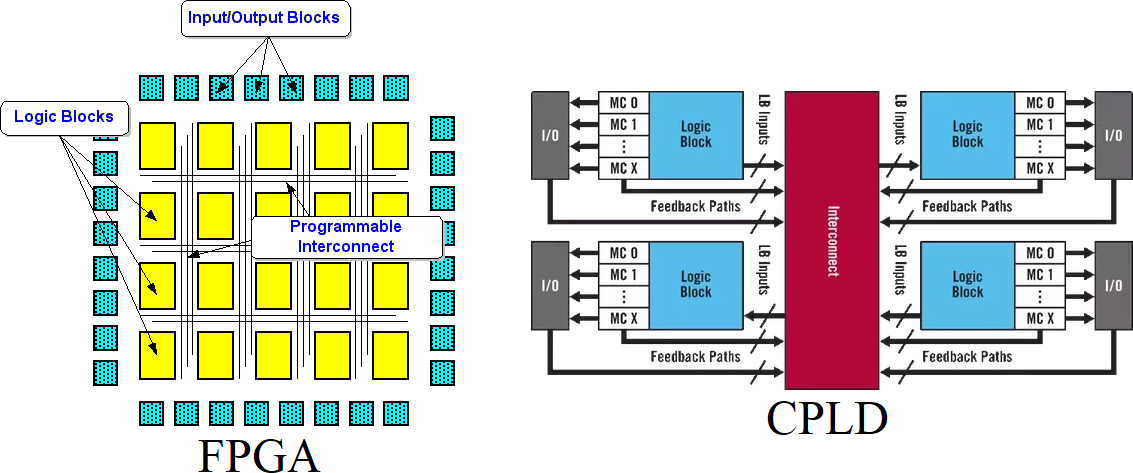
\includegraphics[width=\textwidth]{fpga_vs_cpld_architectures.png}
    \caption{FPGA's architecture (left) vs. CPLD's architecture (right). \href{https://www.quora.com/What-is-the-difference-between-CPLD-and-FPGA/answer/Gregory-James}{Source}}
    \label{figure:3}
  \end{figure}
\end{enumerate}

%%%%%%%%%%%%%%%%%%%%%%%%%%%%%%%%%%%%%%%%%%%%%%%%%%%%%%%%%%%%%%%%%%%%%%%%%%%%%%%%
% Appendix
%%%%%%%%%%%%%%%%%%%%%%%%%%%%%%%%%%%%%%%%%%%%%%%%%%%%%%%%%%%%%%%%%%%%%%%%%%%%%%%%
\section*{Appendix}

No appendix is available in this lab.

%%%%%%%%%%%%%%%%%%%%%%%%%%%%%%%%%%%%%%%%%%%%%%%%%%%%%%%%%%%%%%%%%%%%%%%%%%%%%%%%
% Bibliography
%%%%%%%%%%%%%%%%%%%%%%%%%%%%%%%%%%%%%%%%%%%%%%%%%%%%%%%%%%%%%%%%%%%%%%%%%%%%%%%%
\bibliographystyle{ieeetr}
\bibliography{references}

\end{document}
